\begin{figure}[htbp]
\centering
\begin{tikzpicture}[x=1cm,y=1cm]
\node[anchor=south west,inner sep=0] at (0,0) {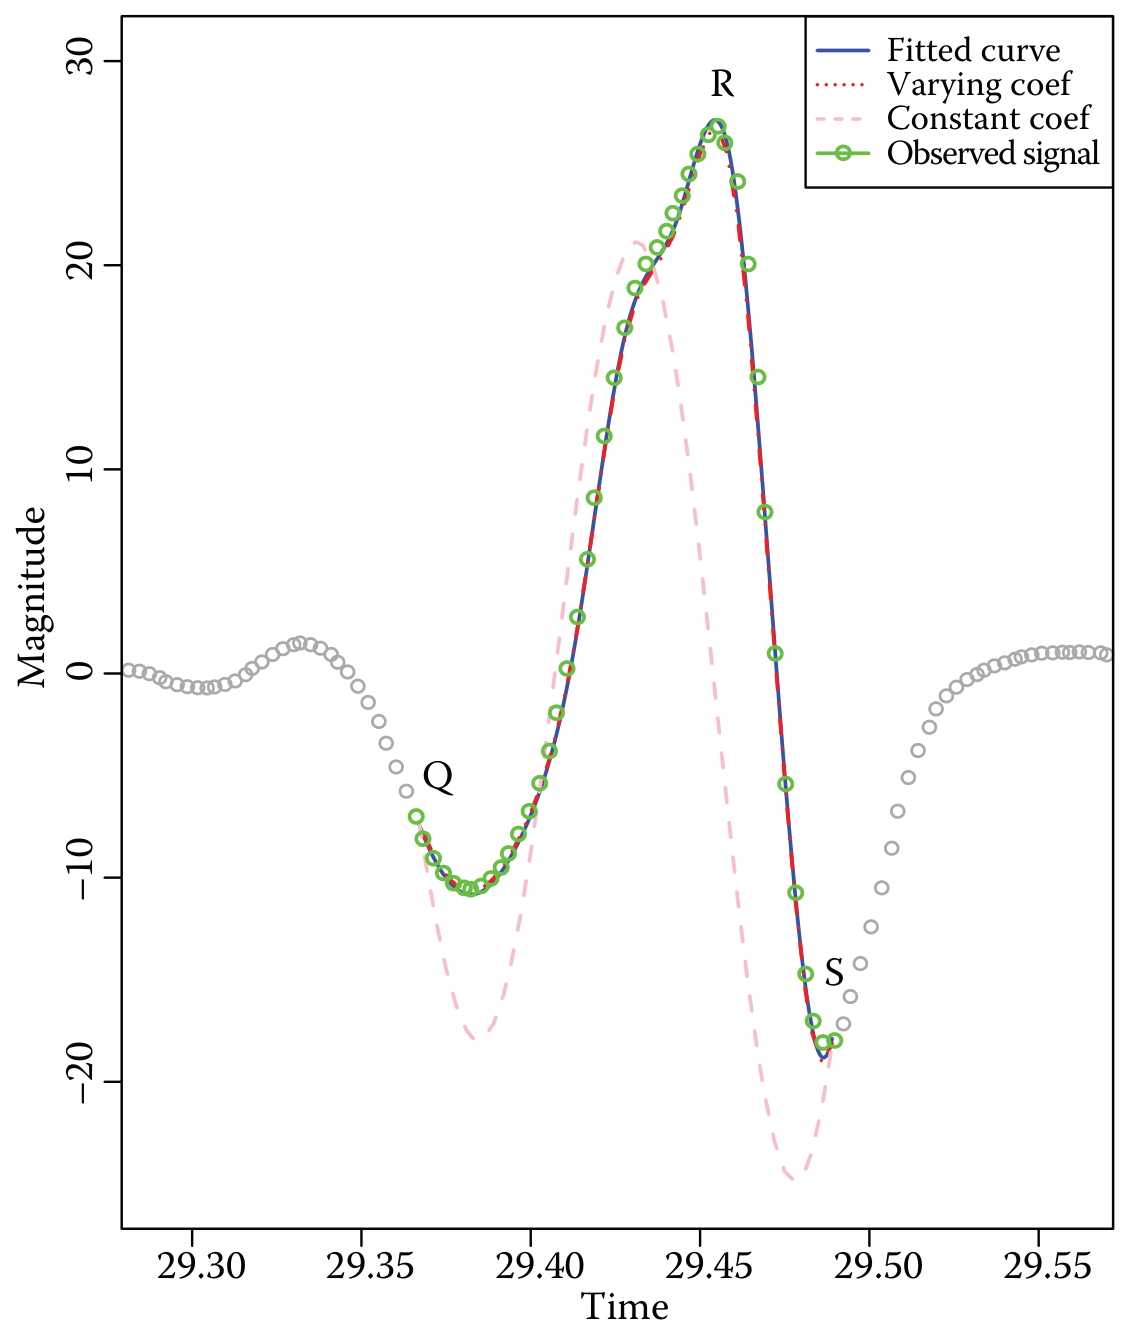
\includegraphics[width=10.5cm]{figures/ch03_fig04_data.png}};
\fill[white] (8.2460,10.7427) rectangle (10.3553,12.2827);
\fill[white] (5.3825,0.0329) rectangle (6.2718,0.4529);
\node[font=\scriptsize,rotate=0,inner sep=0] at (5.8272,0.2429) {时间};
\fill[white] (0.0991,6.0075) rectangle (0.5284,7.7569);
\node[font=\scriptsize,rotate=90,inner sep=0] at (0.3137,6.8822) {幅值};
\node[font=\scriptsize,rotate=0,inner sep=0] at (9.0889,11.9754) {拟合曲线};
\node[font=\scriptsize,rotate=0,inner sep=0] at (9.1335,11.6555) {时变系数};
\node[font=\scriptsize,rotate=0,inner sep=0] at (9.2214,11.3356) {常系数};
\node[font=\scriptsize,rotate=0,inner sep=0] at (9.2714,11.0158) {观测信号};
\end{tikzpicture}
\origfig{4}{时变二阶常微分方程对异常 QRS 波群的拟合曲线。}
\label{fig:ch03-04}
\end{figure}
